\chapter{Theoretical Foundations}\label{ch:theoretical-foundations}


\section{Sheet Metal}\label{sec:sheet-metal}
% Definition
Sheet metal is typically produced through the process of flat rolling various types of metals, resulting in a
characteristic aspect ratio of surface area thickness that typically falls within the range of
0.4\,mm to 6\,mm.
When the value exceeds this particular range, it is classified as a ``plate'', whereas if it falls below the range,
it is classified as a ``foil''
~\cite[p. 405]{groover_fundamentalsmodernmanufacturing_2020}.
% Material
Due to its accessibility, good formability, and sufficient strength for the majority of uses, low-carbon steel is a
regularly used type of sheet metal
~\cite[p. 405]{groover_fundamentalsmodernmanufacturing_2020}.
% Commercial importance
Sheet metals play a vital role in many industries for example automotive and aerospace to reduce the weight of
products~\cite[p. 1]{zheng_reviewformingtechniques_2018}.

\subsection{Sheet Metal Manufacturing}\label{subsec:sheet-metal-manufacturing}
% Manufacturing methods
The process of working with sheet metal is known as sheet-metal press-working and is often done with machine tools
called presses.
Utilizing so called ``punch-and-die tooling'' that is specifically made for these procedures, stamping presses are
employed to complete these processes
~\cite[p. 405]{groover_fundamentalsmodernmanufacturing_2020}.
The punch is a shaped tool that is usually mounted as upper part on the press ram and applies
pressure on the sheet metal to shape it.
The die is a stationary tool that is mounted in the press bed and provides a support surface for
the sheet metal and also defines the shape of the finished
product~\cref{sec:bending}~\cite[p. 412]{groover_fundamentalsmodernmanufacturing_2020}.
\cref{fig:bending-methods} shows the tooling setup together with a sheet metal being bend.
While the term `punch' is quite intuitive, the term ``die'' can cause confusion.
The term `die' is a typically term in metal working to refer to the lower or stationary part of a tooling setup.

Cutting, bending, and drawing are the three main groups of sheet metal forming processes.
While bending and drawing processes are used to mold sheet metal into the desired forms necessary for making certain
parts, cutting is used to separate huge sheets of material into smaller pieces.
~\cite[p. 405]{groover_fundamentalsmodernmanufacturing_2020}.
Drawing involves stretching the metal to create a convex or concave shape
~\cite[p. 416]{groover_fundamentalsmodernmanufacturing_2020}, while bending is ``defined as the straining of the
metal around a straight axis''
~\cite[p. 412]{groover_fundamentalsmodernmanufacturing_2020}.
This study focuses on metal bending and the bending method used in this study (Air Bending) deploys a mixture of
bending and drawing and will be explained in more detail in the next
section~\cite[pp. 416]{groover_fundamentalsmodernmanufacturing_2020}.


\section{Sheet Metal Bending}\label{sec:bending}
% Bending definition and description
Bending is a forming operation that is used to change the shape of a sheet metal by
applying a load to it.
It involves using force to shape the sheet metal into a desired form
~\cite[p. 1]{dib_singleensembleclassifiers_2020}.
The metal is subjected to a load that is greater than its yield strength but less than its ultimate tensile strength
, allowing the metal to be permanently deformed into a different shape.
~\cite[p. 1]{baig_machinelearningprediction_2021}.
% TODO Selbst hergeleitet aber keine Quelle?
This means that a load below the yield strength will not deform the metal, while a load above the utlimate tensile
strength will cause the metal to break.

Sheet metal bending is usually used to produce large quantities of components at low cost in various
industries~\cite[p. 1]{dib_singleensembleclassifiers_2020}.
The metal sheet experiences plastic deformation during the bending process, when the outside fibers are stretched and
the inside fibers are compressed.
As a result, the sheet metal curves in the direction of the applied load.
~\cite[pp. 1--3]{baig_machinelearningprediction_2021}.
The differently loaded cross-sectional areas are separated by a neutral plane in which theoretically no load occurs.
%The bending process creates a neutral plane, which an imaginary surface within the metal sheet where there is
%neither compression nor stretching.
If only the loaded cross-section is considered for simplification, the neutral plane is also referred to as the
neutral axis or neutral line
~\cite[pp. 67]{gustafson1998analytical}.
%It is also called neutral axis or neutral line~\cite[pp. 67]{gustafson1998analytical}.
\cref{fig:neutral-plane} shows the neutral plane after the bending operation, it is
visible, that it is closer to the inside of the bend than to the outside of the bend.
The arrows show where the metal was stretched and where it was compressed.

\begin{figure}[h]
    \begin{tcolorbox}[arc=0pt,boxrule=0.5pt, colback=white]
        \centering
        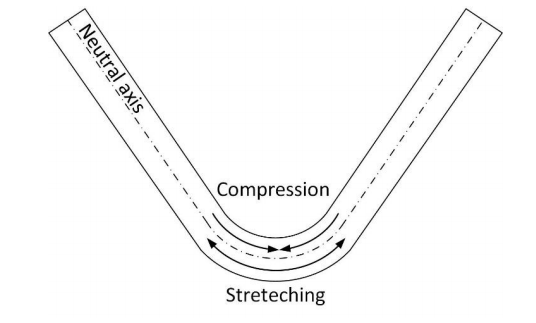
\includegraphics[width=0.6\textwidth]{chap2/images/neutral-plane}
    \end{tcolorbox}
    \caption{Neutral plane and the compression and stretching of a sheet metal
    ~\cite[p. 3]{baig_machinelearningprediction_2021}}
    \label{fig:neutral-plane}
\end{figure}

% TODO How curvature is achieved (keine Quelle?)
The amount of curvature that is achieved in the bending process is determined by the
amount of load applied, the thickness and properties of the metal and the location and length of the neutral plane.
By controlling these factors, it is possible to achieve precise and consistent results in the bending of sheet metal.

\subsection{Air Bending}\label{subsec:air-bending}
In the manufacturing industry, bending sheet metal is a critical process, allowing for the creation of various metal
shapes and configurations.
As can be seen in Groover (2020) V-bending and its variant, Air Bending, are both techniques that utilize punch-and
-die tooling ~\cite[p. 416]{groover_fundamentalsmodernmanufacturing_2020}.
The V-bending process, as shown in Figure~\ref{fig:v-bending}, entails pressing the metal into the shape of the die
to form precise and complex bends.
The die can take various shapes, including U-shaped, Z-shaped, or any other shape required to achieve the desired bend.

In contrast, air bending, as depicted in Figure~\ref{fig:air-bending}, utilizes an open die that only supports the
metal on each side.
This process permits a more extensive range of bend angles since the punch travel distance is not
restricted by the die.
Air bending can also achieve a tighter bend radius compared to V-bending, but it may result in
a slightly rounded bend.

\begin{figure}[h]
    \begin{tcolorbox}[arc=0pt,boxrule=0.5pt, colback=white]
        \centering
        \begin{subfigure}{0.4\textwidth}
            \centering
            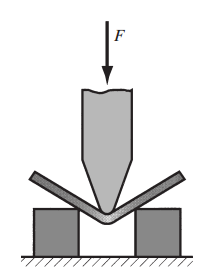
\includegraphics[width=\textwidth]{chap3/images/air-bending}
            \caption{Air bending}
            \label{fig:air-bending}
        \end{subfigure}
        \hfill
        \begin{subfigure}{0.4\textwidth}
            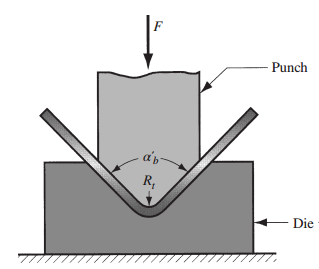
\includegraphics[width=\textwidth]{chap3/images/v-bending}
            \caption{V-Bending}
            \label{fig:v-bending}
        \end{subfigure}
        \hfill
    \end{tcolorbox}
    \caption{Differnt bending methods~\cite[pp. 416]{groover_fundamentalsmodernmanufacturing_2020}}
    \label{fig:bending-methods}
\end{figure}

% Usage of air bending
In the automotive sector, air bending is frequently utilized to create sheet metal components
~\cite[p. 342]{kim_predictionbendallowance_2007}.
Because it is flexible, it can achieve a variety of bending angles with the same punch-and-die tooling, it
is usually the most popular bending technique
~\cite[p. 3]{miranda_formingspringbackprediction_2018}~\cite[p. 1]{cruz_applicationmachinelearning_2021}.

Modern press machines are frequently fitted with "computer numerical control" (CNC) systems, which automatically
regulate the bending process and generate the desired shape.
~\cite[p. 3]{miranda_formingspringbackprediction_2018}
The process parameters are explained in \cref{fig:process_parameters}.

\subsubsection{Spring Back}\label{subsubsec:spring-back}
% How the spring back is created
After the deformation pressure is released, there is still
some elastic energy remaining in the bent part.
As a result, the bent part will partially return to its original
shape, which is known as spring back
~\cite[p. 413--414]{groover_fundamentalsmodernmanufacturing_2020}.

\cref{fig:spring-back} shows the spring back of a metal plate after the punch was removed.
The spring back is determined by the angle of the bent part after the punch is removed compared to the angle when
the punch was still applied.
The solid line shows the metal plate in its original form when the punch was still
applied.
The dashed line shows the metal plate after the punch was removed.

\begin{figure}[h]
    \centering
    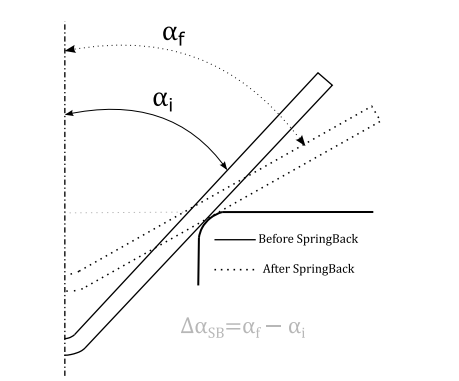
\includegraphics[width=0.5\textwidth]{chap3/images/spring-back}
    \caption{Spring back~\cite[p. 5]{cruz_applicationmachinelearning_2021}}
    \label{fig:spring-back}
\end{figure}

The angle before the spring back is usually denoted as $\alpha_i$ and the angle after spring back as $\alpha_f$.
% Introduce of formula
The spring back ($\Delta \alpha_{SB}$) is therefore the difference between $\alpha_f$ and
$\alpha_i$ as show in equation~\ref*{eq:calculation_springback}~\cite[p. 6]{cruz_applicationmachinelearning_2021}.


\begin{tcolorbox}[arc=0pt,boxrule=0.5pt]
    \begin{equation}
        \delta \alpha_{SB} = \alpha_f - \alpha_i
        \label{eq:calculation_springback}
    \end{equation}
\end{tcolorbox}

To tackle this problem, there are various techniques to compensate for spring back.
One commonly used approach is over bending, wherein the punch angle and radius are fabricated smaller than the
specified angle.
Prerequisite for all compensation methods is that the amount of spring back is known therefore
the accurate prediction of the spring back play an important role in the manufacturing
process ~\cite[p. 114]{groover_fundamentalsmodernmanufacturing_2020}.


\section{Machine Learning}\label{sec:machine-learning}
\cite{muller_introductionmachinelearning_2016} describe machine learning as ``Machine learning is about extracting
knowledge from data.'' and ``it is a research field at the intersection of statistics, artificial intelligence, and
computer science and is also known as predictive analytics or statistical learning.''
~\cite[p. 1]{muller_introductionmachinelearning_2016}.

The purpose of the model is to make predictions or decisions without explicitly requiring programming to do so.
\cite{el2015machine} use programming terms to explain thad ML models rather than being ``hard coded'', are ``soft
coded'', which means that they naturally alter their structure through repetition to increase their performance in
performing the target task ~\cite[pp. 4]{el2015machine}~\cite[pp. 151--170]{koza1996automated}.
``This adaptive process is known as training, and it involves providing the algorithm with input data samples and the
expected outputs, allowing the system to optimize itself to achieve the desired result not only with the training
inputs but also with new, previously unseen data.''
~\cite[pp. 4]{el2015machine}.
The training is the fundamental aspect of \ac{ML} and it can be continuous allowing the algorithm to
learn from new data and its mistakes~\cite[pp. 4]{el2015machine}.

Machine learning algorithms have numerous applications in fields just as example
agriculture (\cite{yoosefzadeh2021application}), computer vision (\cite{hu2020voronoi}) or metal working
(see section~\ref{sec:state-of-research}).

\subsection{Terminology}\label{subsec:terminology}
This study tries to use common terminology for \ac{ML} to make it easier to understand:
To carry out machine learning, a \textit{dataset} (~\cite[p. 3]{zhou_machinelearning_2021}) is required as the
initial foundation.
A dataset is composed of \textit{samples}, with each sample being a single row or observation.
For example, if a dataset contains information about metal sheet bending, each row would represent a single bend.

A \textit{feature} is an individual measurable property or characteristic of the data, and the associated value is
called an \textit{attribute}.
A feature could be, for example, the thickness of a sheet metal component, and the attribute could be 3 mm.
Features used to predict the outcome of a sample are called \textit{independent features} or \textit{input}, while the
outcome feature is referred to as the \textit{dependent feature} or \textit{target}.
In this study, the spring back is the dependent feature, while the other features which will be explained later are
independent features.
The dataset of this study will be explained in~\cref{subsec:dataset-exploration}.

The process of using machine learning algorithms to create a model is called \textit{training} or \textit{fitting}
~\cite[p. 4]{el2015machine}, and the data used for that process is commonly referred to as \textit{training data}.
Usually, the training data is a subset of the whole dataset.
The process of using the model to make predictions on new, unseen data is called
\textit{generalization}
~\cite[pp. 26--27]{muller_introductionmachinelearning_2016}~\cite[p. 4]{zhou_machinelearning_2021}.
The test-train split is described in more detail in section~\ref{subsec:training-test-split}.

The outcome of the learning process is referred to as a \textit{model} that can be used to make predictions on new,
unseen data.\ac{ML} algorithms are also often referred as \textit{learners}.

\subsection{Supervised Learning and Unsupervised Learning}\label{subsec:supervised-learning}
Learning tasks are classified into two types based on whether or not the outcome is already included in the training
data.
There are two types of learning: supervised learning and unsupervised learning.
~\cite[p. 4]{zhou_machinelearning_2021}.

Supervised learning is employed when not only the independent features but also the dependent feature is known.
Since this is the case in the dataset used in this study, supervised learning is the preferred
method
~\cite[p. 2]{muller_introductionmachinelearning_2016}.
To achieve this supervised \ac{ML} algorithms are trained with parts of the dataset, the training data.
Building the training set usually requires human effort but once it is built supervised learning automates the task
and makes it more efficient.
The two main types of supervised learning are classification and regression
~\cite[p. 25]{muller_introductionmachinelearning_2016}, which will be explained in the following section.

\subsection{Classification and Regression}\label{subsec:regression}
Problems that are solved with machine learning can fall in one of two categories: Classifications and regression
problems.
Depending on the nature of the problems different algorithms are performance metrics are used~(see
~\cref{subsec:correctness}).
For classifications the ML model needs to predict a class label from a predefined set of labels which are already
present in the dataset
~\cite[pp. 25--26]{muller_introductionmachinelearning_2016}.
An example could be the prediction of the type of a flower based on its features such as
petal length and width.
The possible outcomes are the different types of flowers, which are the class labels.

On the other hand in regression problems the ML models tries to predict a continuous number
~\cite[pp. 25--26]{muller_introductionmachinelearning_2016}.
An example for a regression problem could be the prediction of the price of a flat based on its features such as
location of rooms and square footage.
The price in ths case is a continuous value, which means that it is not discrete

In this study the goal is to predict the spring back of sheet metal components, which is a continues number and
therefore a regression problem.
One usual problem of regression as well as classification ML models is that they tend to over-fit the training data
which will be explained in the following section.

\subsection{Overfitting and Underfitting}\label{subsec:overfitting-and-underfitting}
The discrepancy between the output predicted by the learning algorithm and the actual output is referred to as the
error.
The error is usually determined on the new for the model unseen samples and therefore is also
called generalization error.
The error calculated on the training set is called empirical error.
~\cite[p. 26]{zhou_machinelearning_2021}.

One of the main goals of Machine Learning is to minimize the generalization error to create a model that performs well
on new, unseen data.
The difficulty is, that the details of new samples are unknown while training the learning algorithm, that means that
only the empirical error can be minimized.
This bears the risk of creating models that perform well on the training data but generalize poorly on new, unseen data.
A usual reason is that the algorithm learns details of the training samples as general properties of the data
which are not true for new samples.
This phenomenon is called overfitting and is the main reason why the generalization error is usually higher than the
empirical error.
The opposite phenomenon is called underfitting and happens when the algorithm fails to learn geneal properties of
the training samples~\cite[p. 26]{zhou_machinelearning_2021}.

Overfitting models are too complex for the amount of data provided and hence do not generalize well, whereas
underfitting models are too simplistic and perform poorly on the training set
~\cite[p. 28]{muller_introductionmachinelearning_2016}.

\cite{badillo2020introduction} makes a good example for overfitting shown in
\cref{fig:overfitting_example}.
The left plot shows a model that is too simple and therefore underfits the data while the most right plot shows a model
that is too complex and therefore overfits the data.
The middle plot shows a model that fits the data well and generalizes well to new samples.

\begin{figure}[h]
    \begin{tcolorbox}[arc=0pt,boxrule=0.5pt]
        \centering
        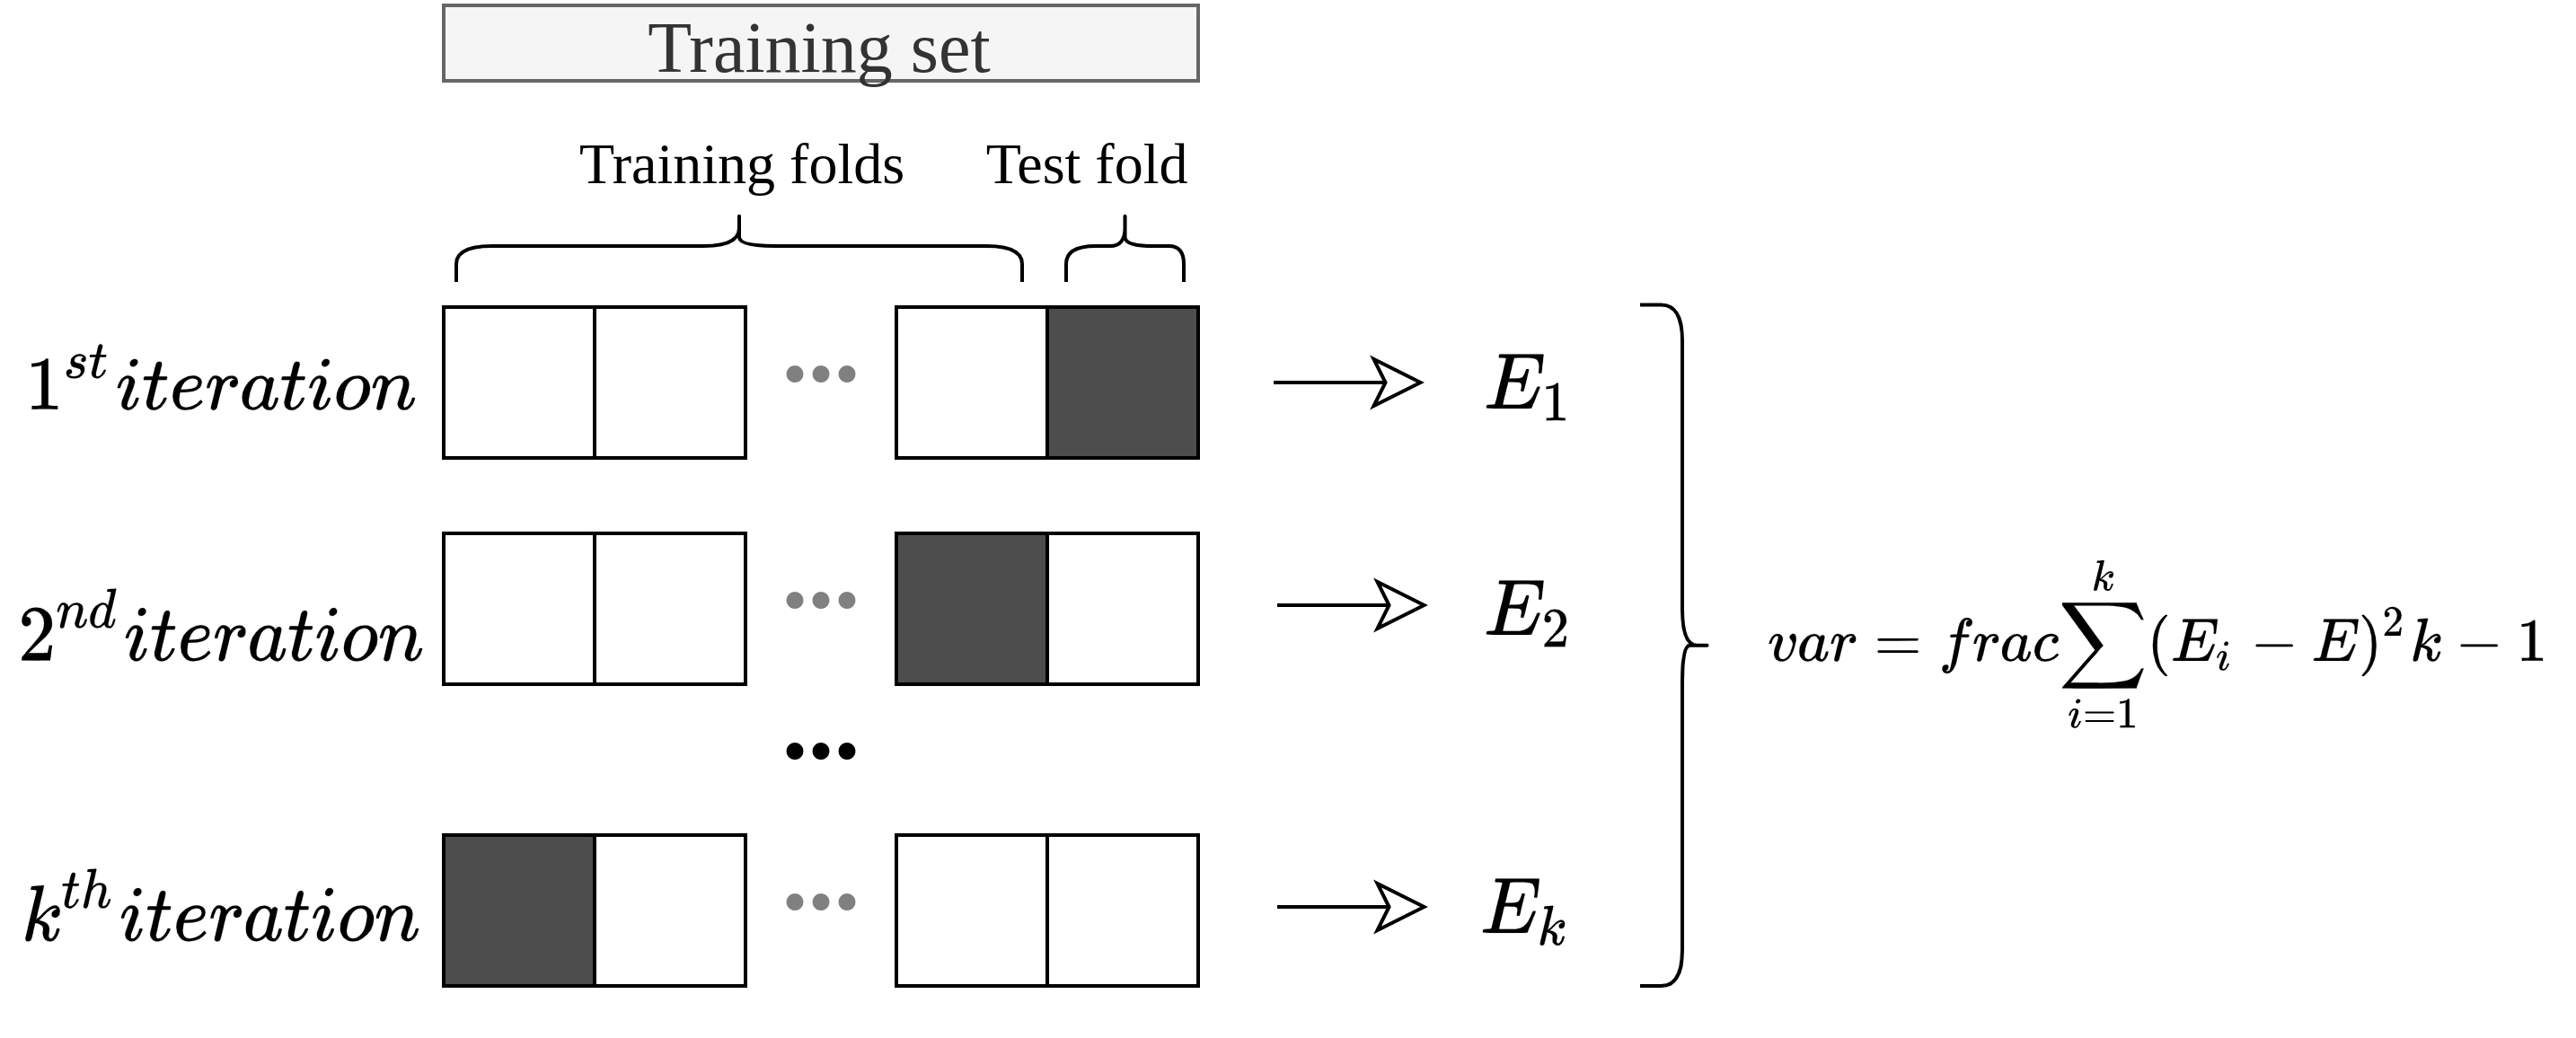
\includegraphics[trim=left botm right top, width=0.9\textwidth]
        {chap2/images/cross_validation}
        \caption{Variance of cross-validation, source:~\cite[p. 260]{muller_introductionmachinelearning_2016}, own
        illustration }
        \label{fig:overfitting_example}
    \end{tcolorbox}
\end{figure}

The goal is to find the simplest model that captures the variability in the
data~\cite[p. 35]{muller_introductionmachinelearning_2016}.
Overfitting and underfitting can result from two different sources of error in the model: bias and variance, which
will be explained in the following section.

\subsection{Bias-Variance Tradeoff}\label{subsec:bias-variance-tradeoff}
% TODO Keine quelle für acuracy und precision
To explain the bias and variance first some terminology is needed.
Accuracy refers usually to the closeness of the model's predictions to the actual values.
Precision refers to the closeness of the model's predictions to each other, meaning how consistent the model's
predictions
are.
Bias can be though of as the opposite of precision and refers to the systematic error in the model's predictions,
meaning how far off the predictions are from the actual values.
~\cite[p. 2]{doroudi2020bias}.
Applying this on the previous \cref{subsec:overfitting-and-underfitting} high bias can result in underfitting, where
the models is too simple to capture the complexity of the data.
Variance on the other hand is the opposite of precision and refers to the variability of the model's predictions when
trained on different subsets of the data
~\cite[p. 2]{doroudi2020bias}.
High variance can result in overfitting, where the model learns the noise in the training data and therefore does not
generalize well to new data (again \cref{subsec:overfitting-and-underfitting}).

% TODO Keine Quelle
Variance and bias are conflicting because they represent two different sources of error.
Error from bias is due to the model being too simple, while error from variance is due to the model being too
complex.
In order to have good generalization performance of the model a small bias and a small variance is favourable.
%The term ``variance'' refers to the variability in the learning performance cause by changes in the training
%set~\cite[p. 51]{zhou_machinelearning_2021}.
\cite{geman1992neural} describe in their paper that the ``price to pay for achieving low bias is high variance''
~\cite[p. 14]{geman1992neural}.
Therefore, as the model becomes more complex, the bias decreases and the variance increases, and vice vers
~\cite[p. 14]{geman1992neural}.
This is known as the bias-variance tradeoff and goal is to find a model that has a low bias and a low variance
and minimized the overall error.

At this point common errors in ML models are explained and the goal of ML models is to minimize the generalization
error.
The following sections explain how to evaluate and improve ML models and how to find the best model for a given
problem.

\subsection{Evaluation and Improvements of Models}\label{subsec:evaluations-and-improvements-of-models}
There are several methods to evaluate and improve ML models.
In the following sections provide explanations for the most important metrics and methods for this study.

\subsubsection{Regression Evaluation Metrics}\label{subsubsec:regression-metrics}
Commonly used metrics for regression models are the \ac{MAE}, Mean Squared Error \ac{MSE} and \ac{RMSE}.
Their formal description is given in the equations~\ref{eq:mae} and~\ref{eq:rmse} where
$e_i$ is the prediction error which is the difference between the predicted value of the model and the actual value.
While $y_i$ is the actual value and $n$ is the number of samples in the testing data set.

The MAE is a measure of the average magnitude of errors in a set of predictions, without considering their direction.
As it returns the same units as the data, it is easy to interpret.
A lower MAE indicates better model performance~\cite[pp. 1248]{chai2014root}.

\begin{tcolorbox}[arc=0pt,boxrule=0.5pt]
    \begin{equation}
        MAE = \frac{1}{n} \sum_{i=1}^{n} |e_i|
        \label{eq:mae}
    \end{equation}
\end{tcolorbox}

The MSE is computed like shown in \cref{eq:rmse}~\cite[p. 1248]{chai2014root} (only the part inside the root) by
determining the average of the squared differences between the predicted and actual values.
%As it is based on squared differences, it is more sensitive to outliers than the MAE
If the predicted responses closely align with the actual responses, the MSE will be low, but if there is a significant
difference between the predicted and actual responses , the MSE will be high~\cite[p. 30]{hastie2009elements}.
The MSE is expressed in squared units of the data, making it difficult to interpret and therefore the RMSE is preferred.

The RMSE measures the average difference between the predicted and actual values and is calculated as the square root
of the MSE.
Its expression is in the same units as the response variable, making it the most popular metric for assessing the
effectiveness of regression models.
The RMSE and respectively the MSE are more sensitive to outliers than the MAE.

\begin{tcolorbox}[arc=0pt,boxrule=0.5pt]
    \begin{equation}
        \label{eq:rmse}
        MSE = \sqrt{\frac{1}{n} \sum_{i=1}^{n} e_i^2}
    \end{equation}
\end{tcolorbox}

\subsubsection{Cross Validation}\label{subsubsec:cross-validation}
% TODO gut genug paraphrasiert?
Cross-validation is a technique for testing a model's performance by training multiple models on different subsets of
data and comparing their performance.
The most frequent type of cross-validation is k-fold cross-validation, which divides the data into k folds and trains
k models, each with one fold serving as the test set and the remainder serving as the training set.
set
~\cite[p. 252--260]{muller_introductionmachinelearning_2016}.
The accuracy of each model is then assessed, and the average accuracy over all k models is used to quantify the model's
generalization performance.
This process helps to reduce the variability in model performance due to the specific choice of training and test
sets, and is therefore considered to be a more stable and reliable way to evaluate the performance of a
model
~\cite[p. 252--260]{muller_introductionmachinelearning_2016}.

Figure~\ref{fig:cross-validation} shows how the cross-validation process and how the variance
is calculated.
It can be seen that the training data set was divided into multiple folds.
The number of folds is denoted as $k$.
One fold is used as test set (grey) while the remaining folds are used as training set (white).
A model is trained on each iteration and the performance is evaluated with a metric denoted as $E$.
Common metrics that can be used for evaluation are $R^2$, $MSE$, $MAE$ and $RMSE$ which are explained in section
\ref{sec:dp1:-correctness} where they are used.

\begin{figure}[h]
    \begin{tcolorbox}[arc=0pt,boxrule=0.5pt]
        \centering
        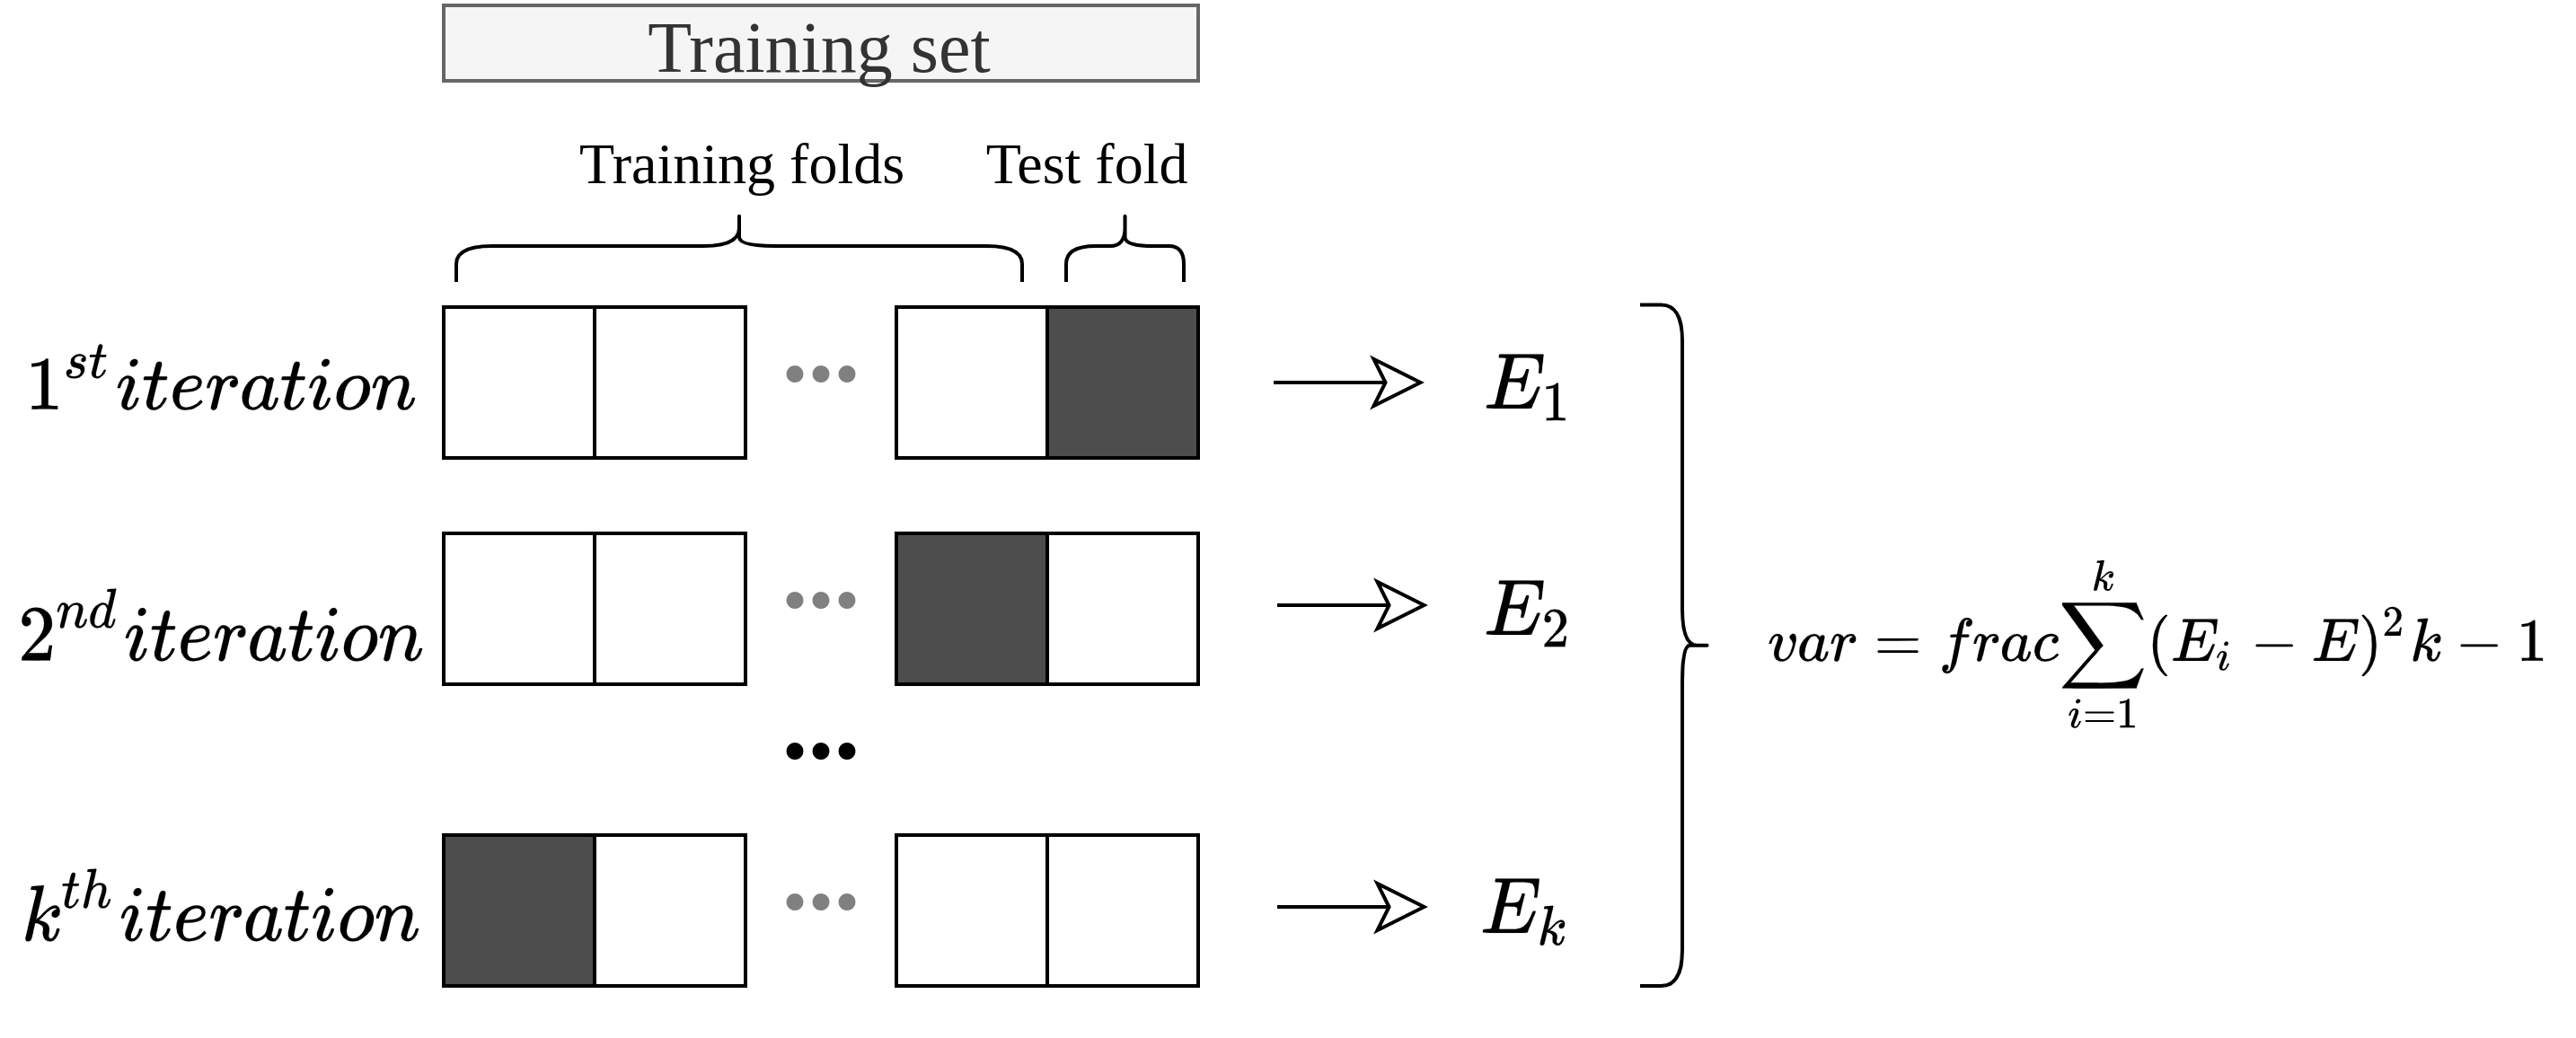
\includegraphics[trim=left botm right top, width=0.9\textwidth]
        {chap2/images/cross_validation}
        \caption{Variance of cross-validation, source:~\cite[p. 260]{muller_introductionmachinelearning_2016}, own
        illustration }
        \label{fig:cross-validation}
    \end{tcolorbox}
\end{figure}

\subsubsection{Grid Search}\label{subsubsec:grid-search}
Each machine learning method has a number of parameters that can be tuned to improve the
performance of the model.
Parameters are often not known in advance and must be tuned to the data.
This is a common task in machine learning and therefore there are standard methods like
grid search to find the best parameters.
Grid search is a method of systematically working through multiple combinations of
parameters (called grid), cross-validating as it goes to determine which tune gives the best
performance
~\cite[p. 260--275]{muller_introductionmachinelearning_2016}.


\section{State of research}\label{sec:state-of-research}
Sheet metals are prone to experience spring back after being bend since their elastic properties.
Therefore, extensive research has already been conducted about spring back behavior in sheet metal forming processes.
~\cite[p. 566]{liu2021deep}.
This chapter presents a non-exhaustive overview of the most important research for this study in the field of
spring back prediction in sheet metal forming processes.
The overview focuses on the application of \ac{ML} methods to predict the spring back.

In recent years, there has been a surge in the adoption of \ac{ML} for various applications related to sheet metal
forming, aiming to achieve optimal manufacturing quality.
Both supervised and unsupervised \ac{ML} methods have been employed in these applications
~\cite[p. 2]{cruz_applicationmachinelearning_2021}.
Current research on mitigating spring back in sheet metal forming often use numerical simulations, most notably
finite element analysis (FEA) to generate the data
~\cite[p. 566]{liu2021deep}.
That means that the data used for training the model is generated by a simulation and not generated with real-life
experiments.

\cite{lingbeek2005development} present two methods for compensating spring back in the deep
drawing process, but conclude that more reliable simulations are needed for industrial applications.
Using a Support Vector Machine, Liu et al. predicted spring back in a micro W-bending process.
When compared to experimental results, they demonstrated high prediction accuracy and generalization performance
~\cite[p. 1]{liu_springbackpredictionforming_2019}.

\cite{dib_singleensembleclassifiers_2020} investigated a variety of \ac{ML} algorithms for predicting spring back and
maximum thinning in
U-channel and square cup forming processes.
The Multilayer Perceptron model was discovered to be the most effective
~\cite[]{dib_singleensembleclassifiers_2020}.
Similarly,~\cite{abdessalem2015probabilistic} compared the performance of a quadratic response surface method (RSM)
and two \ac{SVM} models for determining the best surrogate model for probabilistic sheet metal structure optimization.
The \ac{SVM} models both outperformed the RSM model
~\cite[]{abdessalem2015probabilistic}.

It has to be noted that most of the research including \ac{ML} relies on FEA to generate the data for training and
testing the models.
This is due to the fact that it is time consuming to obtain enough experimental data for
sheet metal forming processes.
Dib et al. observe that virtual tryout implementations continue to rely substantially on human experience to make
crucial decisions.
Furthermore, the use of FEM does not guarantee the elimination of unforeseen faults caused by differences in material
properties, tool geometry, and process parameters
~\cite[p. 2]{dib_singleensembleclassifiers_2020}.

\cite{liu_springbackpredictionforming_2019} used a Support Vector Machine \ac{SVM} to predict the spring back of
micro W-Bending operations~\cite[]{liu_springbackpredictionforming_2019}.
\cite{dib_singleensembleclassifiers_2020} compared different \ac{ML} techniques (logistic regression, SVM, KNN
, ANN, Random Forest, Decision Tree, Naive Bayes, MSP) to predict the spring back and the occurrence of
defects in sheet metal~\cite[p. 1]{dib_singleensembleclassifiers_2020}.
The authors conclude that the MLP and the SVM are the best performing algorithms and
suggest further studies of ML regressions models and kriging regression
models~\cite[p. 13]{dib_singleensembleclassifiers_2020}.

\subsection*{Spring Back Prediction Using ANNs}

Because of their great accuracy and generalization capabilities, \ac{ANN}s are used in sheet metal forming.
~\cite[p. 2]{cruz_applicationmachinelearning_2021}.
\cite{narayanasamy_comparisonregressionartificial_2012a} compared neural network and regression models to predict the
spring back of steel sheet metal during the air bending process.
They discovered that ANN could predict the spring back with greater accuracy
~\cite[]{narayanasamy_comparisonregressionartificial_2012a}.
\cite{inamdar_developmentartificialneural_2000} created an ANN for the air bending process that
predicts both spring back and punch travel in
order to
achieve the desired angle in a single stroke.
~\cite{inamdar_developmentartificialneural_2000}.
\cite{kazan_predictionspringbackwipebending_2009} developed an ANN trained with FEM simulation data to predict the
spring back for the wipe-bending process.

Because \ac{ANN}s need a large amount of data to train the model generating the data
with real machines is a time-consuming process.
Therefore, it is common to use \ac{ANN}s trained with Finite Element Method \ac{FEM}simulation data.